\documentclass{article}

\usepackage{ucs}
\usepackage[utf8x]{inputenc}	% enable utf8
\usepackage[russian]{babel}		% enable russian language
\usepackage[left=1.7cm,right=1.7cm,top=2cm,bottom=2cm,bindingoffset=0cm]{geometry}
\usepackage{mathtools}
\usepackage{graphicx}
\usepackage{listings}
\usepackage{color}

\definecolor{mygreen}{rgb}{0,0.6,0}
\definecolor{mygray}{rgb}{0.5,0.5,0.5}
\definecolor{mymauve}{rgb}{0.58,0,0.82}

\lstset {
    language=C++,
    backgroundcolor=\color{white}, % set backgroundcolor
    basicstyle=\footnotesize, % basic font setting
    captionpos=b, % sets the caption-position to bottom
    extendedchars=\true,
    numbers=left,
    stepnumber=1,
    showstringspaces=false,
    breaklines=true,
    commentstyle=\color{mygreen},    % comment style
    escapeinside={\%*}{*)},          % if you want to add LaTeX within your code
    keywordstyle=\color{blue},       % keyword style
    stringstyle=\color{mymauve},     % string literal style
    basicstyle=\linespread{1.2},
	tabsize=4,
}

\title{Labaratory №2}
\date{}
\author{Beernadsky Gregory, Komarik Zakhar, Shnaider Ksenia}

\begin{document}
\maketitle
\section{Tasks}


\subsection{}
Разработать подпрограмму генерации регулярных и адаптивных сеточных разбиений произвольного отрезка \([a, b]\) в зависимости от числа сегментов разбиения и величины коэффициента разрядки \(r\)
\begin{figure}
	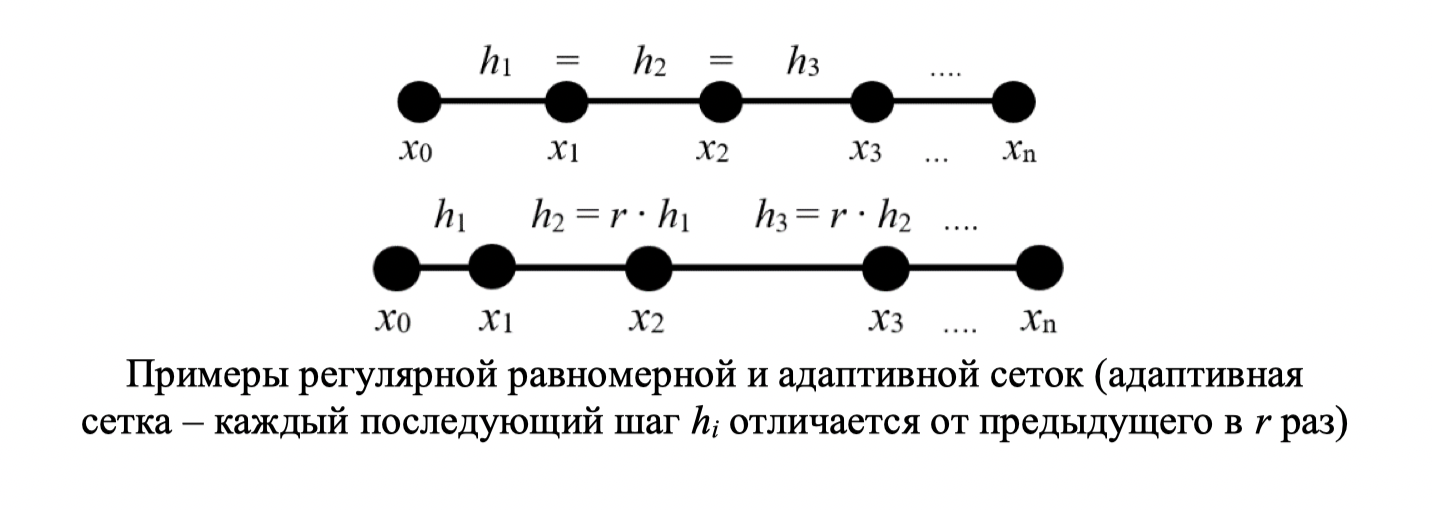
\includegraphics[width=\linewidth, height=7cm]{images/imaget1.png}
	\caption{Взято из учебного пособия}
\end{figure}

\subsection{}
Кусочно-полиномиальная интерполяция. Разработать класс, реализующий интерфейс кубического интерполяционного сплайна с непрерывными первой и второй производными и удовлетворяющего краевым условиям нулевой кривизны \(S'' (a) = S'' (b) = 0\).

\subsection{}
Для набора аналитических функций \(f(x) = x, x^2, x^3, x^4, sin(x)\) провести исследования на вложенных сетках. Для этого задайте шаг h и постройте равномерное сеточное разбиение отрезка \([a, b]\). Получите таблицу значений сплайна и его двух первых производных в точках, которые НЕ совпадают с узловыми (не менее 10). Повторить данные исследования на сетках с шагом \(h/2\) и \(h/4\). Полученные результаты сопоставьте с аналитической оценкой точности сплайн-аппроксимации: если \(f(x)\in C^{k + 1}[a, b]\), \(0 \leq k \leq 3\), то для интерполяционного сплайна \(S(x)\) выполнено \(max _{x\in [a,b] }|f(^{(m)}(x) − S^{(m)}(x)| \leq Ch^{k+1-m} max_{x\in [a,b] }|f^{(m)}(x)|, C - const\) т.е. погрешность аппроксимации ограничена сверху величиной \(O(h^{k+1-m})\) при ограниченной \(m\)-ой производной аппроксимируемой функции. В отчёте привести величину шага \(h\) и соответствующую норму погрешности аппроксимации.

\subsection{}
Выяснить как влияет на вторую производную сгущение сетки к концам отрезка \([a,b]\).

\subsection{}
Сглаживание и аппроксимация МНК. Разработать класс, реализующий интерфейс сглаживающего сплайна. На каждом сегменте разбиения использовать базисную систему финитных функций первого порядка. Сглаживающий сплайн \(g(x)\) строить как решение задачи о минимизации функционала в линейном подпространстве \(\Omega \subset C[a,b] \hspace{1em} \Phi=(1−p)||f(x)−g(x)||^2_2+p||g'(x)||^2_2\)
, где \(p\) – параметр сглаживания.

\subsection{}
Для сильно осциллирующей функции \(f(x)=x|sin(10000x)|\), \(x\) – радианы, на одной диаграмме изобразить интерполяционный и сглаживающий сплайны. Параметр сглаживания \(p\) варьировать от 0 до 1. Использовать равномерную сетку с шагом \(h\) и \(h/2\).

\subsection{}
Выяснить, на что влияет варьирование весовых коэффициентов в дискретном скалярном произведении при построении сглаживающего сплайна.

\section{Solutions}

\subsection{}
\begin{enumerate}
	\item Spliting.hpp
	\begin{lstlisting}
template <typename T = double>
std::vector<Point<T>> spliting(T first,
							   T second,
							   size_t amount,
							   T r = 1.,
							   bool dir = true)
{
	auto left{std::min(first, second)}, right{std::max(first, second)};
	std::vector<Point<T>> grid;
	grid.recerve(amount);
	for (auto current = (dir ? left : right);
		(dir ? right : left) - current > eps<T>;
		current += (step *= r))
			grid.emplace_back({current});
    grid.emplace_back((dir ? right : left));
	return grid;
}
	\end{lstlisting}
\end{enumerate}

\subsection{}
\begin{enumerate}
	\item Splain.hpp
	\begin{lstlisting}
#pragma once

#include <array>
#include <vector>
#include <stdexcept>
#include <utility>

namespace af
{
template <typename T = double> using Point = std::array<T, 3>;
template <typename T = double> using SplainValue = Point<T>;

template <typename T = double> class Splain
{
  public:
    Splain()
    {
      if (!std::is_floating_point<T>::value)
        throw std::logic_error("For normal work use floating types : float, double, long double\n");
    }
    /**
     * first is anchor points
     * second is values of tables function
     */
    virtual void update(std::vector<Point<T>> const &, std::vector<T> const &) = 0;
    /**
     * first is point
     * second is tabel function values
     */
    virtual SplainValue<T> getValue(Point<T> const &) const = 0;
};
} // namespace af

	\end{lstlisting}
	\item CubicInterpolationSplain.hpp
	\begin{lstlisting}
#pragma once

#include "../Splain.hpp"
#include "../../constants.hpp"
#include <algorithm>
#include <cmath>
#include <stdexcept>

namespace af
{
template <typename T = double> class CubicInterpolationSplain : public af::Splain<T>
{
  public:
    void update(std::vector<Point<T>> const &, std::vector<T> const &) override;
    SplainValue<T> getValue(Point<T> const &) const override;

  private:
    /**
     * @brief grid of splain points
     */
    std::vector<Point<T>> grid;
    /**
     * @brief coefficient [a, b, c, d] of cubic interpolation splain
     */
    std::vector<std::array<T, 4>> coefficient;
};
} // namespace af

#include "CubicInterpolationSplain.inl"
	\end{lstlisting}
	\item CubicInterpolationSplain.inl
	\begin{lstlisting}
#include "CubicInterpolationSplain.hpp"

template <typename T>
void af::CubicInterpolationSplain<T>::update(std::vector<af::Point<T>> const &points, std::vector<T> const &fValues)
{
    size_t amountSegment = points.size();

    if (amountSegment-- <= 1)
        throw std::invalid_argument("A few amount of point!");

    this->grid.resize(amountSegment + 1);
    std::copy(points.begin(), points.end(), grid.begin());

    coefficient.resize(amountSegment);

    T current{}, next{}; // h (step)
    std::vector<T> fi(amountSegment - 1);

    // get coefficient [a, b, d] and fi
    for (size_t i = 0; i < amountSegment - 1; ++i)
    {
        current = grid[i + 1][0] - grid[i][0];
        next = grid[i + 2][0] - grid[i + 1][0];

        //  b[i] = 2 * (current + next)
        coefficient[i][1] = 2 * (current + next);

        // a[i + 1] = current
        coefficient[i + 1][0] = current;

        // d[i] = next
        coefficient[i][3] = next;

        fi[i] = 3. * ((fValues[i + 2] - fValues[i + 1]) / next - (fValues[i + 1] - fValues[i]) / current);
    }

    // to forward
    for (size_t i = 1; i < amountSegment - 1; ++i)
    {
        // a[i] / b[i - 1]
        auto buf = coefficient[i][0] / coefficient[i - 1][1];

        // b[i] = a[i] / b[i - 1] * d[i - 1]
        coefficient[i][1] -= buf * coefficient[i - 1][3];

        fi[i] -= buf * fi[i - 1];
    }

    // to back
    // c[amountSegment - 1] = fi[amountSegment - 2] / b[amountSegment - 2]
    coefficient[amountSegment - 1][2] =
        fi[amountSegment - 2] / coefficient[amountSegment - 2][1];
    for (size_t i = amountSegment - 3; i < amountSegment; --i)
        // c[i + 1] = (fi[i] - c[i + 2] * d[i]) / b[i]
        coefficient[i + 1][2] =
            (fi[i] - coefficient[i + 2][2] * coefficient[i][3]) / coefficient[i][1];
    // c[0] = 0.0
    coefficient[0][2] = 0.;

    // coefficient of splain
    for (size_t i = 0; i < amountSegment - 1; ++i)
    {
        current = grid[i + 1][0] - grid[i][0];
        // a[1] = fValues[i]
        coefficient[i][0] = fValues[i];
        // b[i] = (fValues[i + 1] / fValues[i]) / current - (c[i + 1] + 2 * c[i]) * current / 3
        coefficient[i][1] =
            (fValues[i + 1] - fValues[i]) / current - (coefficient[i + 1][2] + 2. * coefficient[i][2]) * current / 3.;
        // d[i] = (c[i + 1] - c[i]) / (current * 3)
        coefficient[i][3] =
            (coefficient[i + 1][2] - coefficient[i][2]) / (current * 3.);
    }

    // last coefficient
    current = grid[amountSegment][0] - grid[amountSegment - 1][0];
    // a[1] = fValues[i]
    coefficient[amountSegment - 1][0] = fValues[amountSegment - 1];
    // b[i] = (fValues[i + 1] / fValues[i]) / current - (c[i + 1] + 2 * c[i]) * current / 3
    coefficient[amountSegment - 1][1] = (fValues[amountSegment] - fValues[amountSegment - 1]) / current -
                                    2. * coefficient[amountSegment - 1][2] * current / 3.;
    // d[i] = (c[i + 1] - c[i]) / (current * 3)
    coefficient[amountSegment - 1][3] = -coefficient[amountSegment - 1][2] / (current * 3.);
}

template <typename T> af::SplainValue<T> af::CubicInterpolationSplain<T>::getValue(af::Point<T> const &point) const
{
    size_t amountSegment = grid.size();
    if (amountSegment-- <= 1)
        throw std::invalid_argument("Grid is so small!");

    for (size_t i = 0; i < amountSegment; ++i)
    {
        if (point[0] > grid[i][0] && point[0] < grid[i + 1][0] ||
            fabs(point[0] - grid[i][0]) < eps<T> ||
            fabs(point[0] - grid[i + 1][0]) < eps<T>)
        {
            T distance = fabs(point[0] - grid[i][0]);
            return  {
                        coefficient[i][0] + coefficient[i][1] * distance + coefficient[i][2] * distance * distance + coefficient[i][3] * distance * distance * distance,

                        coefficient[i][1] + 2. * coefficient[i][2] * distance + 3. * coefficient[i][3] * distance * distance,

                        2. * coefficient[i][2] + 6. * coefficient[i][3] * distance
                    };
        }
    }
    throw std::domain_error("Point out of the domain");
}
	\end{lstlisting}
\end{enumerate}

\end{document}
